\documentclass{standalone}

\usepackage{xcolor}

\definecolor{myblue}{HTML}{377EB8}
\definecolor{myred}{HTML}{E41A1C}
\definecolor{myviolet}{HTML}{984EA3}

\usepackage{tikz}
\usepackage{pgfplots}
\pgfplotsset{compat=newest}

\usetikzlibrary{patterns}

\usepackage{lmodern}
\SetSymbolFont{letters}{bold}{OML}{cmbr}{bx}{it}
\renewcommand{\familydefault}{\sfdefault}

\usepackage{sansmathfonts}

\begin{document}
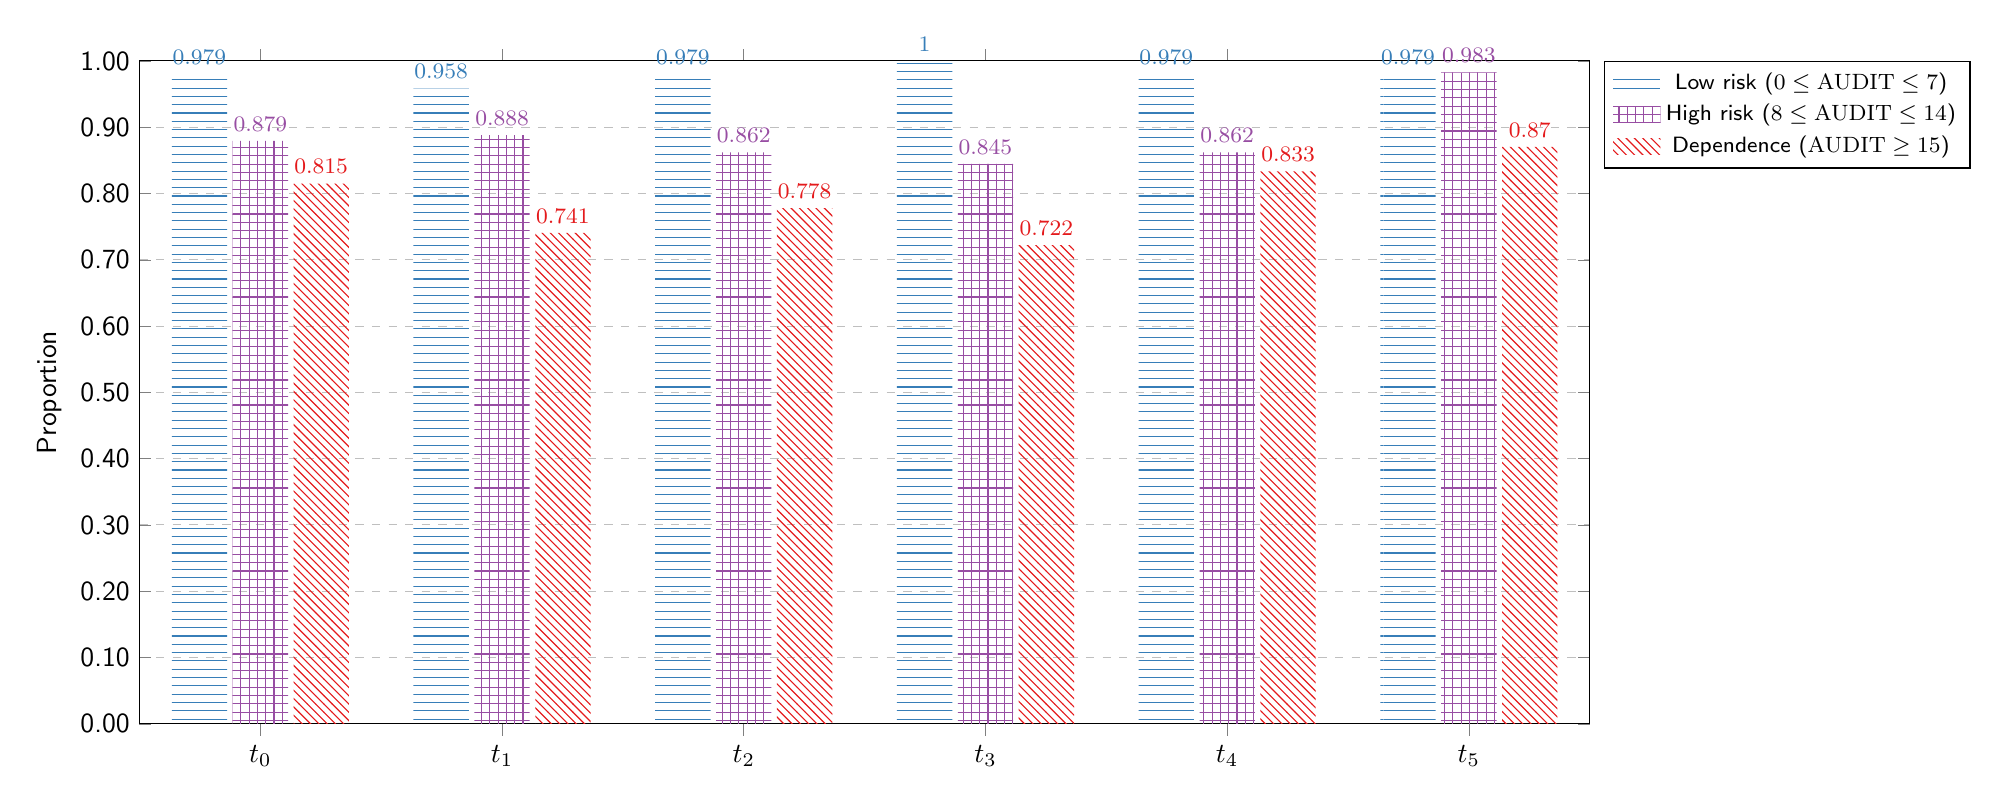
\begin{tikzpicture}
	\begin{axis}[
			ybar,
			ymin=0.00,
			ymax=1.00,
			ytick={0.00,0.10,0.20,0.30,0.40,0.50,0.60,0.70,0.80,0.90,1.00},
			yticklabels={0.00,0.10,0.20,0.30,0.40,0.50,0.60,0.70,0.80,0.90,1.00},
			ylabel = {Proportion},
			symbolic x coords = {
				$t_{0}$,
				$t_{1}$,
				$t_{2}$,
				$t_{3}$,
				$t_{4}$,
				$t_{5}$
			},
			xtick = data,
			width = 20cm,
			height = 10cm,
			ymajorgrids = true,
			grid style = dashed,
			nodes near coords={
				\pgfmathprintnumber[fixed, precision=3]{\pgfplotspointmeta}
			},
			nodes near coords align={vertical},
			nodes near coords style = {font = \footnotesize},
			bar width = 20pt,
			legend image code/.code = {%
				\draw[#1, draw = none] (0cm, -0.1cm) rectangle (0.6cm, 0.1cm);
			},
			legend style = {
				font = \footnotesize,
				at = {(1.01,1)},
				anchor = north west,
			},
		]
		\addplot[pattern = horizontal lines, pattern color=myblue, draw = none, nodes near coords style={color = myblue}] coordinates {
			($t_{0}$, 0.9791667)
			($t_{1}$, 0.9583333)
			($t_{2}$, 0.9791667)
			($t_{3}$, 1.00000000)
			($t_{4}$, 0.9791667)
			($t_{5}$, 0.9791667)
		};
		\addplot[pattern = grid, pattern color = myviolet, draw = none, nodes near coords style={color = myviolet}] coordinates {
			($t_{0}$, 0.8793103)
			($t_{1}$, 0.887931)
			($t_{2}$, 0.862069)
			($t_{3}$, 0.8448276)
			($t_{4}$, 0.862069)
			($t_{5}$, 0.9827586)
		};
		\addplot[pattern = north west lines, pattern color = myred, draw = none, nodes near coords style={color = myred}] coordinates {
			($t_{0}$, 0.8148148)
			($t_{1}$, 0.7407407)
			($t_{2}$, 0.7777778)
			($t_{3}$, 0.7222222)
			($t_{4}$, 0.8333333)
			($t_{5}$, 0.8703704)
		};
		\legend{Low risk ($0 \leq \mathrm{AUDIT} \leq 7$), High risk ($8 \leq \mathrm{AUDIT} \leq 14$), Dependence ($\mathrm{AUDIT} \geq 15$)}
	\end{axis}
\end{tikzpicture}
\end{document}
